Los routers de Wi-Fi generalmente ofrecen dos bandas con frecuencias distintas: una de 2.4 GHz y otra de 5 GHz.

\textbf{2.4 GHZ} tiene más rango, pero es más lenta y tiene más interferencia. \textbf{5 GHz} tiene menos rango, pero es más rápida y tiene menos interferencia.

\begin{figure}[H]
  \centering
  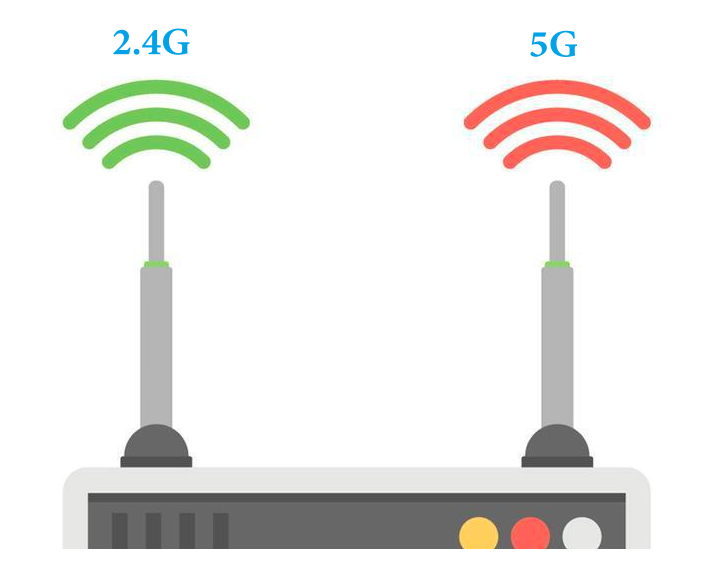
\includegraphics[scale=0.3]{imagenes/wifi.png}
  \caption{Wi-Fi 2.4 GHz y 5 GHz\cite{utecwifi}}
\end{figure}
